\chapter{The Underlying Idea of a Hybrid Solver}

The core idea behind a hybrid solver is to alternate between classical processes and QPU-based solutions, enabling the handling of larger problems than those constrained by the limits outlined in Section \ref{sec:qpu-res}.

A common feature of current hybrid implementations is the necessity to partition or, more generally, subdivide the original problem into a set of tractable subproblems. 
This approach allows the ``difficult'' component of the problem to be solved by leveraging quantum acceleration, while the CPU is tasked with aggregating the solutions.
Several strategies for implementing a hybrid solver can be found in the literature.

\paragraph{Branch\&Bound} Viewing the possible assignments as a tree, as illustrated in Figure \ref{fig:assignment}, the search methodology described in this technique involves exploring a hopefully narrow subset of branches and selecting promising paths using heuristics (Bound phase). 
At each level, one of the possible variables is fixed to reduce the remaining subset (Branch phase).

Branch\&Bound has been applied as a partitioning methodology for QUBO problems in \cite{QBNB}.

\begin{figure}
    \centering
    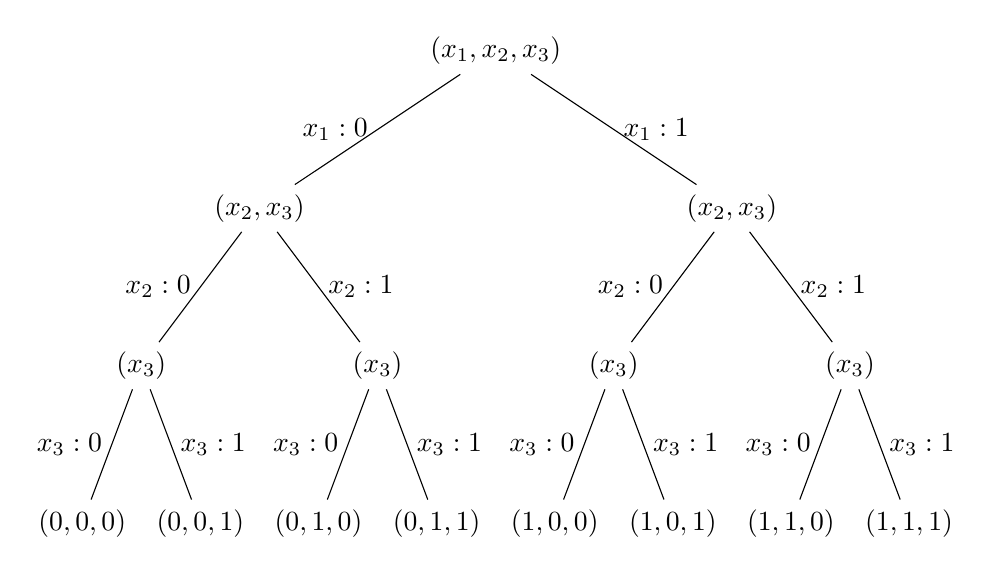
\begin{tikzpicture}[
        level distance=2cm,
        level 1/.style={sibling distance=6cm},
        level 2/.style={sibling distance=3cm},
        level 3/.style={sibling distance=1.5cm},
    ]
        \node {$(x_1, x_2, x_3)$}
        child { node {$(x_2, x_3)$}
            child { node {$(x_3)$}
            child { 
                node {$(0,0,0)$}
                edge from parent node[left] {$x_3:0$}
            }
            child { 
                node {$(0,0,1)$}
                edge from parent node[right] {$x_3:1$}
            }
            edge from parent node[left] {$x_2:0$}
            }
            child { node {$(x_3)$}
                child { 
                    node {$(0,1,0)$}
                    edge from parent node[left] {$x_3:0$}
                }
                child { 
                    node {$(0,1,1)$}
                    edge from parent node[right] {$x_3:1$}
                }
                edge from parent node[right] {$x_2:1$}
            }
            edge from parent node[left] {$x_1:0$}
        }
        child { node {$(x_2, x_3)$}
            child { node {$(x_3)$}
                child { 
                    node {$(1,0,0)$}
                    edge from parent node[left] {$x_3:0$}
                }
                child { 
                    node {$(1,0,1)$}
                    edge from parent node[right] {$x_3:1$}
                }
                edge from parent node[left] {$x_2:0$}
            }
            child { node {$(x_3)$}
                child { 
                    node {$(1,1,0)$}
                    edge from parent node[left] {$x_3:0$}
                }
                child { 
                    node {$(1,1,1)$}
                    edge from parent node[right] {$x_3:1$}
                }
                edge from parent node[right] {$x_2:1$}
            }
            edge from parent node[right] {$x_1:1$}
        };
    \end{tikzpicture}
    \caption{Example of a complete exploration for a problem with three binary variables.}
    \label{fig:assignment}
\end{figure}

\paragraph{Local Search} The solution produced by the QPU for the problem, or a subset of it, can be combined with classical local search methods. 
Local search involves considering the optimization problem as a graph, where each node corresponds to an assignment of the optimization variables and hence a value of the objective function. 
From a given solution, local search explores the neighbourhood to check whether the current state corresponds to a minimum. 
The neighbourhood of a node is defined as the set of states reachable with a maximum number of changes in the assignment, predetermined in advance. 

For example, considering only binary variables and a neighbourhood of distance one, this consists of all assignments that require changing the value of only one optimization variable in the current state.
Local search is a widely used technique in the literature, with several algorithms developed for its implementation. 
A significant drawback common to many procedures is that local minima are difficult to overcome. 

For this reason, combining it with adiabatic quantum computing can be advantageous, as the tunnelling effect can be exploited to converge more quickly towards the global minimum, as described in Section \ref{sec:AQC}.

Before developing proprietary technology, D-Wave proposed this approach for solving large-scale QUBO problems\cite{hybridsearch}, using purely quantum solvers in combination with TabuSearch algorithm\cite{tabusearch}.

\paragraph{Local Embedding} To mitigate the problem size, the possibility of more directly addressing the CSP has been explored\cite{localembedding}. 
Before converting the problem into QUBO form, the embedding is performed separately for the objective function and individual constraints. 
The results are then combined to ensure that the assignment satisfies the problem's requirements.

Although this approach can be interesting, its application is more limited than the other methodologies mentioned.
For instance, in the SVM problem, the CSP formulation consists of: 

\begin{itemize} 
	\item A single, small constraint, Equation \ref{eq:svm-c2}; 
	\item An objective function that dominates the problem's dimensions, Equation \ref{eq:svm-obj}. 
\end{itemize}

This implies that even reducing the problem size would not yield significant benefits. 
This consideration applies to cases where the complexity of the objective function greatly exceeds the complexity of the constraints, which often occurs in CSP formulations.

\paragraph{Proposed Methodology} The partitioning methodology proposed in this thesis focuses on the algebraic properties of the QUBO matrix, which will be discussed in detail in Section \ref{sec:prop}. 
The goal is to maximize the use of the QPU, delegating only the aggregation of partial results to the CPU.

\section{Algebraic Properties of QUBO Problems}\label{sec:prop}

Section \ref{sec:AQC} outlined the general structure of a QUBO problem. 

$$\min X^TQX$$ 

Where $X$ is the column vector of optimization variables with dimension $(n \times 1)$, $X^T$ is the transposed vector with dimension $(1 \times n)$, and $Q$ is the upper triangular square matrix with dimension $n \times n$.

Taking a problem with $n=6$ as an example, the matrix formulation takes the form:

\begin{equation}
    \begin{bmatrix}
        x_1 & x_2 & x_3 & x_4 & x_5 & x_6
    \end{bmatrix}
    \begin{bmatrix}
        q_{11} & q_{12} & q_{13} & q_{14} & q_{15} & q_{16} \\
        0 & q_{22} & q_{23} & q_{24} & q_{25} & q_{26} \\
        0 & 0 & q_{33} & q_{34} & q_{35} & q_{36} \\
        0 & 0 & 0 & q_{44} & q_{45} & q_{46} \\
        0 & 0 & 0 & 0 & q_{55} & q_{56} \\
        0 & 0 & 0 & 0 & 0 & q_{66}
    \end{bmatrix}
    \begin{bmatrix}
        x_1 \\
        x_2 \\
        x_3 \\
        x_4 \\
        x_5 \\
        x_6
    \end{bmatrix}
\end{equation}

The explicit equation describing the problem is:

\begin{multline}
    x_1^2q_{11} + x_1x_2q_{12} + x_2^2q_{22} + x_1x_3q_{13} + x_2x_3q_{23} + x_3^2q_{33} + \\ 
    + x_1x_4q_{14} + x_2x_4q_{24} + x_3x_4q_{34} + x_4^2q_{44} + \\ 
    + x_1x_5q_{15} + x_2x_5q_{25} + x_3x_5q_{35} + x_4x_5q_{45} + x_5^2q_{55} + \\ 
    + x_1x_6q_{16} + x_2x_6q_{26} + x_3x_6q_{36} + x_4x_6q_{46} + x_5x_6q_{56} + x_6^2q_{66}
    \label{eq:whole6}
\end{multline}

The structure of the QUBO problem suggests the possibility of subdividing it into four subproblems of identical dimensions:

\begin{equation}
    \begin{bmatrix}
        x_1 & x_2 & x_3 & | & x_4 & x_5 & x_6
    \end{bmatrix}
    \begin{bmatrix}
        q_{11} & q_{12} & q_{13} & | & q_{14} & q_{15} & q_{16} \\
        0 & q_{22} & q_{23} & | & q_{24} & q_{25} & q_{26} \\
        0 & 0 & q_{33} & | & q_{34} & q_{35} & q_{36} \\
        - & - & - & - & - & -  & - \\
        0 & 0 & 0 & | & q_{44} & q_{45} & q_{46} \\
        0 & 0 & 0 & | & 0 & q_{55} & q_{56} \\
        0 & 0 & 0 & | & 0 & 0 & q_{66}
    \end{bmatrix}
    \begin{bmatrix}
        x_1 \\
        x_2 \\
        x_3 \\
        - \\
        x_4 \\
        x_5 \\
        x_6
    \end{bmatrix}
\end{equation}

It is therefore necessary to verify the feasibility of decomposition by analyzing the results of the subproblems and recombining them to obtain Equation \ref{eq:whole6}.

\paragraph{Subproblem 1}
By dividing the variables into two partitions ($P_1=\{x_1,x_2,x_3\}$ and $P_2=\{x_4,x_5,x_6\}$), the upper-left submatrix of $Q$ (hereafter referred to as $\operatorname{UL}$) forms the following problem:

\begin{equation*}
    P_1^T\operatorname{UL}P_1=
    \begin{bmatrix}
        x_1 & x_2 & x_3
    \end{bmatrix}
    \begin{bmatrix}
        q_{11} & q_{12} & q_{13} \\
        0 & q_{22} & q_{23} \\
        0 & 0 & q_{33}
    \end{bmatrix}
    \begin{bmatrix}
        x_1 \\
        x_2 \\
        x_3 \\
    \end{bmatrix}
\end{equation*}

Expanding this, the equation becomes:

\begin{equation}
 x_1^2q_{11} + x_1x_2q_{12} + x_2^2q_{22} + x_1x_3q_{13} + x_2x_3q_{23} + x_3^2q_{33}
    \label{eq:UL}
\end{equation}

\paragraph{Subproblem 2}
Defining the upper-right submatrix as $\operatorname{UR}$, we obtain the following subproblem:

\begin{equation}
    P_1^T\operatorname{UR}P_2=
    \begin{bmatrix}
        x_1 & x_2 & x_3
    \end{bmatrix}
    \begin{bmatrix}
        q_{14} & q_{15} & q_{16} \\
        q_{24} & q_{25} & q_{26} \\
        q_{34} & q_{35} & q_{36}
    \end{bmatrix}
    \begin{bmatrix}
        x_4 \\
        x_5 \\
        x_6
    \end{bmatrix}
    \label{eq:ur}
\end{equation}

This expands to:

\begin{multline}
    x_1x_4q_{14} + x_2x_4q_{24} + x_3x_4q_{34} + x_1x_5q_{15} + x_2x_5q_{25} + \\ 
    + x_3x_5q_{35} + x_1x_6q_{16} + x_2x_6q_{26} + x_3x_6q_{36} 
    \label{eq:UR}
\end{multline}

\paragraph{Subproblem 3} The bottom-left submatrix ($\operatorname{BL}$) consists entirely of zero coefficients. 
Therefore, the result of $P_2^T\operatorname{BL}P_1$ is always zero.

\begin{equation*}
    \begin{bmatrix}
        x_4 & x_5 & x_6
    \end{bmatrix}
    \begin{bmatrix}
        0 & 0 & 0 \\
        0 & 0 & 0 \\
        0 & 0 & 0
    \end{bmatrix}
    \begin{bmatrix}
        x_1 \\
        x_2 \\
        x_3
    \end{bmatrix}
\end{equation*}

\paragraph{Subproblem 4} From the remaining part of $Q$, referred to as $\operatorname{BR}$, we obtain:

\begin{equation*}
    \begin{bmatrix}
        x_4 & x_5 & x_6
    \end{bmatrix}
    \begin{bmatrix}
        q_{44} & q_{45} & q_{46} \\
        0 & q_{55} & q_{56} \\
        0 & 0 & q_{66}
    \end{bmatrix}
    \begin{bmatrix}
        x_4 \\
        x_5 \\
        x_6
    \end{bmatrix}
\end{equation*}

This expands to:

\begin{equation}
 x_4^2q_{44} + x_4x_5q_{45} + x_5^2q_{55} + x_4x_6q_{46} + x_5x_6q_{56} + x_6^2q_{66}
    \label{eq:BR}
\end{equation}

\paragraph{Solution Aggregation} By summing Equations \ref{eq:UL}, \ref{eq:UR} and \ref{eq:BR}, it is evident that the result is equivalent to Equation \ref{eq:whole6}.

This algebraic property of the QUBO matrix allows the problem to be decomposed and the subproblems to be solved independently before recombining the solutions to achieve the final result.